\documentclass[10pt]{article}
\usepackage[margin=2.2cm]{geometry}
\usepackage{amsmath,amssymb,booktabs,longtable,graphicx,hyperref,array}
\usepackage[T1]{fontenc}
\usepackage[utf8]{inputenc}
\hypersetup{colorlinks=true,linkcolor=blue,urlcolor=blue,citecolor=blue}
\graphicspath{{../results/plots/}}
\emergencystretch=3em
% ---- single-point settings, edited by hand / scripts/set_doi.py ----
\newcommand{\pubdate}{29 September 2026}% publication date: to be set to the date the author gives
\newcommand{\zenododoi}{10.5281/zenodo.23051520}% reserved Zenodo DOI: placeholder until the author provides it

\title{Two certified sum-of-radii circle packings exceeding the Packomania values\\ listed on 29 September 2026,
an exact large-$N$ verifier for the first autocorrelation inequality,\\ and documented negative results}
\author{Elian Alfonso L\'opez Preciado\\ Independent Researcher, Le\'on, Guanajuato, M\'exico\\
\texttt{alfonsolopezelian@gmail.com}}
\date{Preprint, \pubdate\ (computations and record checks: 28--29 September 2026)}

\begin{document}
\maketitle

\begin{abstract}
We study three extremal problems with a common workflow: a search stack (GPU and CPU stages, a sparse sequential-LP local solver, an
evolutionary loop, a high-precision Newton polish) and an \emph{independent} verifier that certifies every reported number in exact
rational arithmetic and in 60-digit arithmetic, in fresh processes.
(i) For the maximum sum of radii of $n$ disjoint circles in the unit square, we exhibit certified packings for $n=120$ and $n=250$
whose sums of radii, 5.7773030974449 and 8.3899735328377, \emph{exceed the values listed in the Packomania ``csqv'' table when we downloaded it on
29~September 2026 at 21:32 (UTC$-6$)} (5.776999746200 and 8.389775077490; gains $3.03\cdot10^{-4}$ and $1.98\cdot10^{-4}$). Both are rigid
($3n$ active constraints, positive multipliers) and are structurally different from the listed configurations. This table changes several times a day:
three other packings of ours ($n=150,188,200$) that were ahead of the table in the morning were overtaken the same day, so these two statements are
time-stamped comparisons, not claims of ``best known''.
(ii) For the first autocorrelation inequality we give an exact-arithmetic verifier (no floating-point FFT) that certifies step functions with up to
$N=38{,}400$ pieces in seconds, and we show that plain coarse-to-fine upsampling stalls at 1.506525 while \emph{partial re-melting} of a smooth surrogate
reaches a certified 1.505275 ($N=19{,}200$): better than the first AlphaEvolve bound (1.50530) but above the later 1.50317 and 1.50287, hence not a record.
(iii) We document matched-only cases ($n=26,\dots,40$ for the sum of radii; 35 point-spreading instances), a tie ($n=110$), a precision artifact ($n=27$) and an overshoot of float scores by up to $5\cdot10^{-11}$.
\end{abstract}

\section{Introduction}
Packomania \cite{packomania} maintains tables of best-known packings. Two of its tables are used here: ``csqv'' (variable-radius circles in a square,
maximising the sum of radii) and ``csq'' (equal circles in a square, equivalently maximising the minimum distance of $n$ points). The csqv problem
was recently used as a benchmark for LLM-guided program evolution \cite{alphaevolve,tttdiscover}, and for $n\ge100$ its table is updated
many times a day by many contributors (the page's update log names about sixteen contributors between 23 July and 29 September 2026). Our data show how fast:
59 rows changed between our downloads of 28 September and 29 September (09:24), and 236 further rows by 15:00.
\textbf{Caveat used throughout:} every comparison with Packomania states the time of the download it refers to; ``ahead'' means ``exceeds the value listed at that time'' and
says nothing about later states of the table.

\paragraph{Contributions.} (a) Certified packings for $n=120$ and $n=250$ exceeding the csqv values listed at 2026-09-29 21:32 (UTC$-6$) (Sec.~\ref{sec:large}), with exact sums, rigidity evidence, symmetry-aware structure comparison with the listed configurations, and files in Packomania's \texttt{.pck} format that pass a from-scratch third-party validator with zero tolerance.
(b) An exact verifier for the first autocorrelation inequality that scales to $N=38{,}400$ without floating-point FFT (Sec.~\ref{sec:c}).
(c) The observation that plain upsampling stalls on a rigid vertex while partial re-melting escapes it (Sec.~\ref{sec:c}); we state plainly that the resulting bound is not a record.
(d) Negative and neutral results: matched-only cases, overtaken cases, a tie, the $n=27$ margin artifact and the float-score overshoot (Sec.~\ref{sec:small}).

\section{Problems and references}
\paragraph{A. Sum of radii (csqv).} Variables $(x_i,y_i,r_i)_{i\le n}$; constraints $r_i\le x_i\le1-r_i$, $r_i\le y_i\le1-r_i$,
$(x_i-x_j)^2+(y_i-y_j)^2\ge(r_i+r_j)^2$; maximise $\sum_ir_i$. Reference: the 12-decimal table \texttt{https://www.packomania.com/csqv/txt/sumradii.txt} (each download is time-stamped;
per-$n$ coordinate files \texttt{csqv<n>.txt} were downloaded for the structure comparisons; none of these files is redistributed with this paper, see Sec.~\ref{sec:repro}). The first AlphaEvolve values
$n=26$: 2.635862 and $n=32$: 2.937944 and their successors 2.635983 and 2.939572 are quoted from \cite{tttdiscover}; the Packomania values at $n=26,32$ are 2.635983084919 and 2.939572771205.
\paragraph{B. Point spreading (csq).} Maximise $\min_{i<j}\|p_i-p_j\|$ over $p_i\in[0,1]^2$; reference \texttt{csq/txt/distance.txt} (12 decimals, 2026-09-28). Optimality is proven for $n\le30$.
\paragraph{C. First autocorrelation inequality.} For a step function with $N$ equal pieces and heights $a_i\ge0$ on $[-\tfrac14,\tfrac14]$,
$R(a)=2N\max_mc_m/(\sum_ia_i)^2$ with $c_m=\sum_{i+j=m}a_ia_j$ upper-bounds the constant $C_1$ ($f{*}f$ is piecewise linear with vertices $h c_m$, $h=1/2N$).
Published bounds, from Table~2 of Yuksekgonul et al.\ \cite{tttdiscover} (arXiv:2601.16175, accessed 2026-09-29): best human 1.50973 (Matolcsi--Vinuesa, 2010), AlphaEvolve 1.50530 \cite{alphaevolve},
AlphaEvolve V2 1.50317, TTT-Discover 1.50287 (30{,}000 pieces; the text of that paper states $C_1\le1.50286$).

\section{Verification}\label{sec:verify}
\paragraph{Independent verifier (\texttt{verify/}).} It imports nothing from the search code. It parses the decimal text of a JSON certificate exactly and checks every constraint
in exact rational arithmetic and in 60-digit \texttt{mpmath}, as separate fresh processes. For problem A every radius is shrunk by $\varepsilon=10^{-12}$ before checking, the
shrunk configuration must satisfy all constraints with violation $\le0$, and the \emph{certified} score is $\sum_i(r_i-\varepsilon)$ (about $n\cdot10^{-12}$ below the exact value); the verifier also reports the raw
(unshrunk) score of the same file. All pairs are checked (never neighbour lists; a test plants an overlap between far-apart indices at $n=120$). For problem C the maximum of the autoconvolution is computed exactly in integers by two algorithms with no shared code (Sec.~\ref{sec:c}).
\paragraph{Third-party validator for \texttt{.pck} files (\texttt{validator/validate\_pck.py}).} Written from scratch, standard library only, it reads a Packomania-layout file
(largest radius, author, then \texttt{x y r} by increasing radius, unit square centred at the origin \cite{packomania}), and checks with zero tolerance in exact integer arithmetic that every circle lies inside the square,
that all $\binom n2$ pairs satisfy $d^2\ge(r_i+r_j)^2$, that line~1 is the largest radius and the order is increasing, and recomputes the sum of radii. It also counts contacts within $3\cdot10^{-12}$ (csqv submissions must have at least $3n$ of them \cite{packomania}).
Tests show it accepts our files and rejects a copy in which one circle is shifted by $10^{-9}$ or one radius is increased by $10^{-9}$.
\paragraph{Consequence for the listed records.} Applying the same validator to Packomania's \emph{listed} $n=120$ and $n=250$ configurations (converted to \texttt{.pck} layout) gives exactly $3n$ contacts within $3\cdot10^{-12}$ but fails the zero-tolerance
overlap check by $\sim10^{-13}$ in squared distance (their coordinates carry 12 decimals). Our \texttt{.pck} files, which carry the $10^{-12}$ radius shrink, pass with zero tolerance and also have exactly $3n$ contacts within $3\cdot10^{-12}$.

\section{Methods}
Local solvers: SLSQP with analytic Jacobians (small $n$), and for $n\ge60$ a sparse sequential LP: with unit vectors $u_{ij}$ the LP $\max\sum\delta r$ subject to
$d_{ij}+u_{ij}\cdot(\delta_i-\delta_j)-r_i-r_j-\delta r_i-\delta r_j\ge0$, exact wall constraints and a trust region $|\delta|\le\Delta$. Since the Euclidean distance is convex in the centres,
every LP-feasible step is truly feasible, iterates stay feasible and $\sum r$ increases monotonically; a pair whose gap exceeds $(2\sqrt2+2)\Delta$ cannot be violated inside the trust region, so
restricting the LP to a neighbour list is exact for that step (tested against brute force). It is 6--20$\times$ faster than dense SLSQP. For fixed centres the optimal radii are an exact LP.
Global search: multistart, basin hopping (jitter, reinsert smallest circles into the largest voids, cluster jitter, swap radii), CMA-ES and DE over centres, an evolutionary loop (tournament selection, line-cut
crossover, niching by radius signature, elitism, migration), a GPU stage (PyTorch; thousands of starts with Adam on an annealed penalty, float32 exploration and float64 refinement, chunked pairwise terms; random, hexagonal-with-vacancies
and radius-graded starts) whose top-$k$ are polished on the CPU, and an optional diagonal-mirror symmetric mode. \emph{Polish:} the active set is identified and minimum-norm Newton steps are iterated to residual $\lesssim10^{-50}$;
for large $n$ the linear solves are in float64 and the residuals in 60-digit arithmetic (iterative refinement, 8--13 digits per step). GPU numbers are screening scores only; nothing counts until the CPU verifier certifies a polished file.
Runs are seedable, checkpointed and resumable. For problem C: a log-sum-exp surrogate with decreasing temperature $\tau$ (Adam, float64 FFT convolution on the GPU), sequential LP polish for $N\le2400$, multilevel continuation and \emph{re-melting} (Sec.~\ref{sec:c}).

\section{Small $n$ and neutral results}\label{sec:small}
\paragraph{Sum of radii, $n=26,\dots,40$ and point spreading.} All 15 sum-of-radii values and all 35 point-spreading values ($n=10,15,20,25,30$ and $31,\dots,60$) reproduce the 12-decimal Packomania values (exact raw values of the sum-of-radii packings within $\sim5\cdot10^{-12}$; point-spreading gaps $\le4.9\cdot10^{-13}$), each with a certificate passing both verifier backends. No improvement. Selected ablation results are in Table~\ref{tab:abl}. \emph{Time budgets are per run and differ between groups} (configured limit / measured wall-clock including process start-up, column ``elapsed'' of Table~\ref{tab:abl}): sum-of-radii CPU pilots at $n=26$ (12 workers) 360\,s / 361--383\,s; at $n=32$ (12 workers) 300\,s / 310--318\,s; GPU pilots at $n=26,32$ (one GPU plus 10 CPU polishing workers) 300\,s / 302--310\,s; point-spreading ablations at $n=40,50$ (12 workers) 120\,s / 120--141\,s; baselines 25\,s or 240\,s; CPU pilots at $n=100$ (11 workers) 600\,s / 600--601\,s; GPU-large pilot at $n=100$ (6 polishing workers) 300\,s / 335\,s (a round takes about 85\,s, so it stopped after the round that crossed the limit). Runs are therefore equal-budget only within a CPU group, and the GPU pilots had a somewhat smaller budget than the CPU pilots at $n=26$ (300\,s vs.\ 360\,s). The 30 runs of Table~\ref{tab:abl} took 7{,}530\,s $=125.5$\,min in total (per run 25--601\,s). Results: at $n=26$ basin hopping, the evolutionary loop and GPU multistart reach the record basin, CPU multistart stops at 2.635977, CMA-ES and DE over centres are worse by $3$--$5\cdot10^{-3}$.
\begin{table}[h]\centering
\begin{center}\resizebox{.95\linewidth}{!}{\begin{tabular}{lllll}
\hline
run & elapsed\_s & best\_score & gap\_to\_record & time\_to\_best\_s \\
\hline
abl\_B\_n40\_bh & 125 & 0.188175522 & +3.151e-13 & 34 \\
abl\_B\_n40\_cmaes & 122 & 0.188068435 & -1.071e-04 & 44 \\
abl\_B\_n40\_evo & 120 & 0.188175522 & +3.151e-13 & 52 \\
abl\_B\_n40\_ms & 125 & 0.188175522 & +3.148e-13 & 49 \\
abl\_B\_n50\_bh & 126 & 0.166377924 & -1.487e-04 & 28 \\
abl\_B\_n50\_cmaes & 122 & 0.166377923 & -1.487e-04 & 51 \\
abl\_B\_n50\_evo & 141 & 0.166454626 & -7.195e-05 & 112 \\
abl\_B\_n50\_ms & 136 & 0.166526577 & -4.497e-13 & 67 \\
base\_B\_n10\_ms & 25 & 0.421279544 & -9.670e-14 & 1 \\
base\_B\_n15\_ms & 25 & 0.341081377 & +1.087e-13 & 2 \\
base\_B\_n20\_ms & 25 & 0.286611652 & -3.186e-13 & 2 \\
base\_B\_n25\_ms & 26 & 0.250000000 & -2.220e-16 & 2 \\
base\_B\_n30\_ms & 26 & 0.224502965 & +8.804e-14 & 3 \\
base\_A\_n26\_ms & 243 & 2.631936898 & -4.046e-03 & 52 \\
gpu\_bh\_A\_n26 & 302 & 2.635983085 & -1.385e-12 & 72 \\
gpu\_bh\_A\_n32 & 302 & 2.939572771 & +1.358e-12 & 104 \\
gpu\_large\_A\_n100 & 335 & 5.256014790 & -7.730e-03 & 86 \\
gpu\_ms\_A\_n26 & 310 & 2.635983085 & +1.074e-12 & 28 \\
gpu\_ms\_A\_n32 & 308 & 2.939572771 & +1.998e-12 & 40 \\
A\_n26\_bh & 361 & 2.635983085 & -6.870e-13 & 11 \\
A\_n26\_cmaes & 363 & 2.633035229 & -2.948e-03 & 25 \\
A\_n26\_de & 383 & 2.631129248 & -4.854e-03 & 331 \\
A\_n26\_evo & 368 & 2.635983085 & +5.480e-12 & 42 \\
A\_n26\_ms & 367 & 2.635977395 & -5.690e-06 & 12 \\
A\_n32\_bh & 314 & 2.939572771 & +1.332e-12 & 149 \\
A\_n32\_evo & 310 & 2.939572771 & +2.726e-12 & 118 \\
A\_n32\_ms & 318 & 2.939572771 & +1.329e-12 & 195 \\
A\_n100\_bh & 601 & 5.254888638 & -8.856e-03 & 198 \\
A\_n100\_evo & 600 & 5.259979380 & -3.765e-03 & 191 \\
A\_n100\_ms & 601 & 5.217176132 & -4.657e-02 & 398 \\
\hline
\end{tabular}
}\end{center}
\caption{Pilot, baseline and ablation runs (A = sum of radii, B = point spreading; ms = multistart, bh = basin hopping, gpu = GPU stage; gaps versus the table of 2026-09-28/29; ``elapsed'' = measured wall-clock per run in seconds, including process start-up; time\_to\_best in seconds; the 30 runs total 7{,}530\,s $=125.5$\,min).}\label{tab:abl}
\end{table}
\paragraph{Float scores overshoot.} Scores from the search (LP repair accepts primal infeasibility $\sim10^{-9}$) can exceed the true value by up to $5\cdot10^{-11}$: the $n=39$ float score 3.248110798226 is $5.1\cdot10^{-11}$ above the listed value, but the exact value of that packing is 3.2481107981734 ($-1.6\cdot10^{-12}$). Only certified values are reported.
\paragraph{The $n=27$ margin artifact.} Our exact sum for $n=27$ is 2.685978684225346, $2.7\cdot10^{-11}$ above the listed 2.685978684198. Matching the two configurations with the Hungarian algorithm under the eight symmetries of the square shows that they are the \emph{same packing}
(maximum deviation $1.4\cdot10^{-12}$; our radii are larger by $1.0\cdot10^{-12}$ on average): the listed radii carry a safety margin of $\approx10^{-12}$ per circle. We do not claim it.

\section{Large $n$ for the sum of radii}\label{sec:large}
\paragraph{Results.} Table~\ref{tab:large} lists the 20 certified packings with $n\ge100$ against the table downloaded on 2026-09-29 at 21:32 (UTC$-6$) (raw exact score of the same file; all packings are rigid: $3n$ active constraints, $3n$ unknowns, full rank, positive multipliers).
\begin{table}[h]\centering
{\footnotesize\begin{tabular}{rllll}
\hline
$n$ & ours (raw exact) & listed record & gap & verdict \\
\hline
100 & 5.260274528761 & 5.263744441843 & $-3.47e-03$ & behind \\
110 & 5.531919536406 & 5.531919536401 & $+4.51e-12$ & tie \\
116 & 5.674350310252 & 5.676573137511 & $-2.22e-03$ & behind \\
120 & 5.777303097445 & 5.776999746200 & $+3.03e-04$ & AHEAD \\
130 & 6.022051095314 & 6.022424077079 & $-3.73e-04$ & behind \\
138 & 6.200571369870 & 6.201196207424 & $-6.25e-04$ & behind \\
139 & 6.222197558817 & 6.224048511183 & $-1.85e-03$ & behind \\
140 & 6.247177080673 & 6.248286289975 & $-1.11e-03$ & behind \\
150 & 6.476386129402 & 6.478189273051 & $-1.80e-03$ & behind \\
159 & 6.661302273433 & 6.663891763480 & $-2.59e-03$ & behind \\
160 & 6.685419110014 & 6.686377484769 & $-9.58e-04$ & behind \\
170 & 6.900527317039 & 6.901615116068 & $-1.09e-03$ & behind \\
180 & 7.099028311558 & 7.099941756488 & $-9.13e-04$ & behind \\
188 & 7.255065345063 & 7.256806779802 & $-1.74e-03$ & behind \\
200 & 7.489453882662 & 7.493815304616 & $-4.36e-03$ & behind \\
250 & 8.389973532838 & 8.389775077490 & $+1.98e-04$ & AHEAD \\
275 & 8.793750914926 & 8.799100032873 & $-5.35e-03$ & behind \\
297 & 9.142259326074 & 9.147139780469 & $-4.88e-03$ & behind \\
300 & 9.191033307299 & 9.192717162187 & $-1.68e-03$ & behind \\
301 & 9.205800667824 & 9.206706957124 & $-9.06e-04$ & behind \\
\hline
\end{tabular}
}
\caption{Certified sum of radii vs.\ the local copy of the Packomania table (\texttt{results/large\_n\_summary.md}; checks are logged in \texttt{results/record\_check\_20260929\_213247.txt}). Positive gap $=$ ahead of the listed value at that time.}\label{tab:large}
\end{table}
\paragraph{The two packings exceeding the listed values.}
\begin{center}\small\begin{tabular}{lll}\hline
 & $n=120$ & $n=250$\\\hline
our exact sum (raw) & 5.77730309744486381328 & 8.38997353283768227131\\
certified sum (shrink $10^{-12}$) & 5.77730309732486381328 & 8.38997353258768227131\\
listed value (2026-09-29 21:32) & 5.776999746200 & 8.389775077490\\
gain (raw $-$ listed) & $+3.034\cdot10^{-4}$ & $+1.985\cdot10^{-4}$\\
active / unknowns / rank & 360 / 360 / 360 & 750 / 750 / 750\\
min.\ KKT multiplier & 0.196 & 0.160\\
\texttt{.pck} validator (zero tolerance) & passed & passed\\
circles within $10^{-6}$ / $10^{-3}$ of listed ones$^*$ & 0 / 12 & 0 / 129\\
max / median deviation$^*$ & $4.3\cdot10^{-2}$ / $5.5\cdot10^{-3}$ & $6.3\cdot10^{-2}$ / $9.2\cdot10^{-4}$\\\hline
\end{tabular}\end{center}
{\footnotesize $^*$ best of the 8 square symmetries, optimal one-to-one assignment of circles; deviation $=\max(|\Delta x|,|\Delta y|,|\Delta r|)$.}\par
Both packings are therefore \emph{different} from the listed ones (contrast $n=27$, where 27/27 circles match to $10^{-12}$): the gains are about six orders of magnitude larger than any safety-margin effect $n\cdot10^{-12}$ (ratios $2.5\cdot10^{6}$ for $n=120$ and $7.9\cdot10^{5}$ for $n=250$, with $n\cdot10^{-12}=1.2\cdot10^{-10}$ and $2.5\cdot10^{-10}$). The overlay (Fig.~\ref{fig:overlay}) shows for $n=120$ the same overall architecture with a rearranged region; for $n=250$ about half of the circles lie within $10^{-3}$ of a listed circle. The packings were still ahead in every download we made after first finding them ($n=120$: 10:39, 15:46, 19:02, 21:32; $n=250$: 15:46, 19:02, 21:32).
\begin{figure}[h]\centering
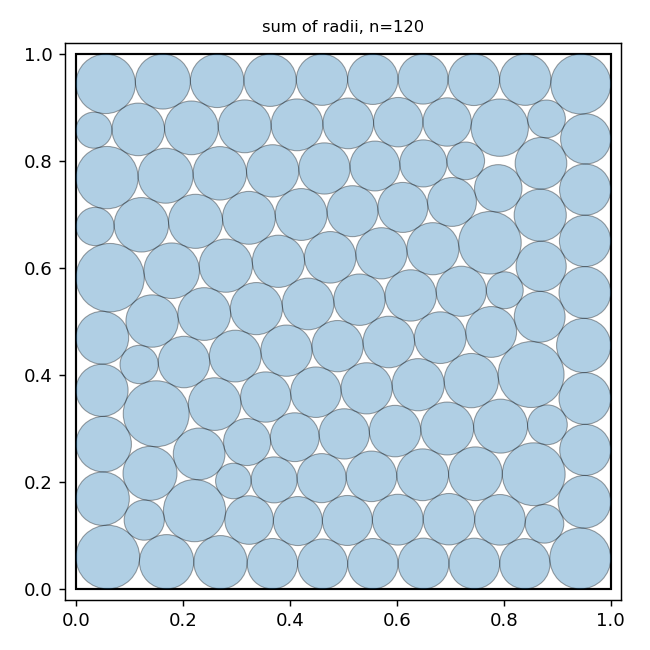
\includegraphics[width=.32\linewidth]{packing_A_n120.png}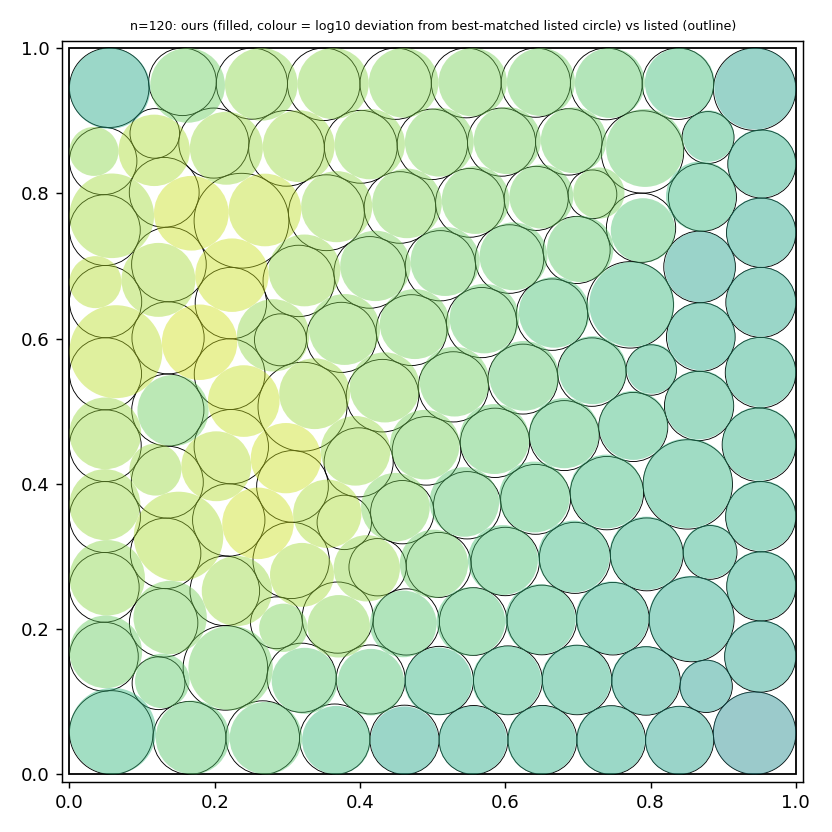
\includegraphics[width=.32\linewidth]{overlay_n120.png}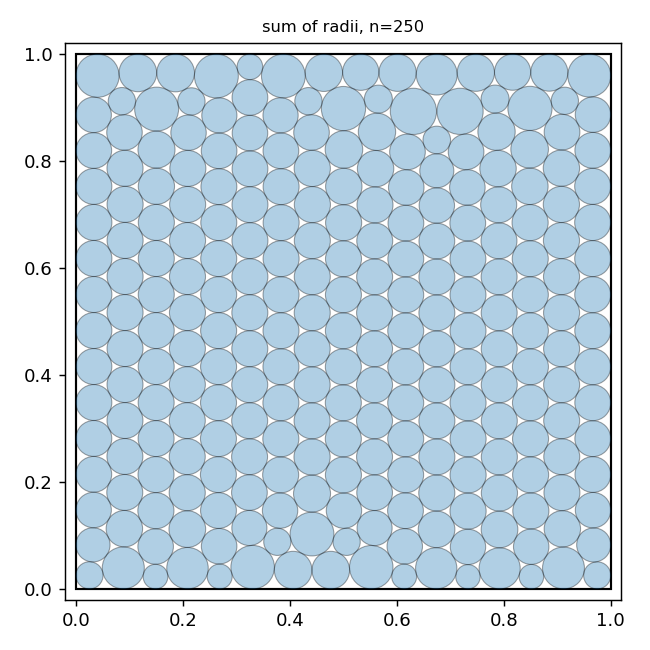
\includegraphics[width=.32\linewidth]{packing_A_n250.png}
\caption{Left: certified $n=120$ packing. Middle: overlay of ours (filled, colour $=\log_{10}$ deviation) and the listed configuration (outline) under the best square symmetry. Right: certified $n=250$ packing.}\label{fig:overlay}
\end{figure}
\paragraph{Overtaken, tied and behind.} The packings for $n=150,188,200$ were ahead of the 09:24 table by $1.4\cdot10^{-4}$, $6.3\cdot10^{-4}$, $2.6\cdot10^{-3}$. By 15:00 the listed values had risen by $1.94\cdot10^{-3}$, $2.37\cdot10^{-3}$ and $6.99\cdot10^{-3}$ respectively (listed value at 15:46 minus listed value at 09:24, computed from the two saved snapshots; the download at 15:00 had read identical values for these three $n$). Our packings are therefore \emph{now behind} the 21:32 table by $1.80\cdot10^{-3}$, $1.74\cdot10^{-3}$ and $4.36\cdot10^{-3}$ (Table~\ref{tab:large}); they are reported as behind and not claimed. $n=110$ ties the listed value ($+4.5\cdot10^{-12}$). All other tested $n$ ($100$--$301$) are behind by $3.7\cdot10^{-4}$ to $5.35\cdot10^{-3}$ (the largest deficit, $n=275$, is $-5.349\cdot10^{-3}$).
\paragraph{What worked.} At $n=100$ (CPU pilots: 11 workers, 600\,s limit each, elapsed 600--601\,s; GPU-large pilot: 300\,s limit, elapsed 335\,s, i.e.\ a smaller budget than the CPU methods; all four runs are in Table~\ref{tab:abl}) the evolutionary loop (5.25998) beat the GPU stage (5.25602), basin hopping (5.25489) and multistart (5.2172); a later main run of the evolutionary loop (four 300\,s chunks, 20\,min) stalled at 5.260275; the successful runs at $n=120,250$ used the evolutionary loop seeded with distinct GPU basins. A diagonal-mirror symmetric mode recovers symmetric records at small $n$ (all top candidates at $n=27$ equal the record after two minutes) but was clearly worse at $n=100$ (best 5.2327); only 4 of our 15 certified packings for $n\in[26,40]$ have a mirror symmetry.

\section{Problem C: exact verification to $N=38{,}400$ and re-melting}\label{sec:c}
\paragraph{Exact verification at scale.} The certified quantity is $R=2N\max_mc_m/(\sum a_i)^2$ with $c_m$ an exact integer (heights scaled by their common denominator). Two independent exact algorithms (\texttt{verify/ac1.py}): Kronecker substitution (all heights packed into one big integer with slots wider than $\log_2(N\max A^2)$, squared with exact big-integer multiplication, slots unpacked) and int64 limb convolution (20-bit limbs, direct \texttt{np.convolve}, every partial sum $<2^{63}$, limbs recombined in Python integers). No floating-point FFT is used. $N=38{,}400$ certifies in about 12\,s with the two backends agreeing to 30 digits; tests cover slot-carry adversaries and equality of the direct, Kronecker and limb algorithms (design in \texttt{docs/verifier\_scaling.md}).
\paragraph{Plain upsampling stalls.} A converged coarse solution upsampled by repetition returns exactly the same value at every level (600 $\to$ 38{,}400: 1.506525181): the optimum is a rigid vertex (the finer grid adds as many active rows as variables), so no first-order descent direction exists. Independent restarts reproduce the plateau (600 pieces, 512 restarts: 1.506526; from scratch $N=300$: 1.5082, $N=1200$: 1.5094, $N=2400$: 1.514). Symmetric profiles are useless ($f{*}f(0)=\int f^2\ge2(\int f)^2$).
\paragraph{Partial re-melting.} At each doubling, or repeatedly at one level, the surrogate is restarted at a large temperature ($\tau_0=3\cdot10^{-3}$--$3\cdot10^{-2}$) from the current solution with 3--10\,\% multiplicative noise and cooled again (Adam on the GPU, 40 stages of 1000 steps). Certified bounds (exact, both backends):
\begin{center}\small\begin{tabular}{rl|rl}\hline $N$ & certified $R$ & $N$ & certified $R$\\\hline
50 & 1.517069339 & 1200 & 1.505817557\\ 95 & 1.511771199 & 2400 & 1.505932519\\ 150 & 1.510256733 & 4800 & 1.505337678\\ 200 & 1.509353547 & 9600 & 1.505296230\\ 300 & 1.508212622 & 19200 & \textbf{1.505274644}\\ 600 & 1.506525181 & 38400 & 1.505274644\\\hline\end{tabular}\end{center}
Each row is the result of one run (the one kept for that $N$), not a running best over $N$, so the sequence is not monotone (for example $R$ at $N=2400$ is above $R$ at $N=1200$): a $2N$-piece step function can always reproduce an $N$-piece one (repeat every height twice), so the optimum over $2N$ pieces is never worse than over $N$, but an individual run need not find it. Hotter restarts helped most; gains shrank to $\sim10^{-5}$ per melt and stalled at $N=19{,}200$ and $38{,}400$. This is better than the best human value (1.50973) and than the first AlphaEvolve bound (1.50530) but $2.0\cdot10^{-3}$ and $2.4\cdot10^{-3}$ \emph{above} AlphaEvolve V2 (1.50317) and the 30{,}000-piece value (1.50287): \textbf{it is not a record} and we make no improvement claim.
\begin{figure}[h]\centering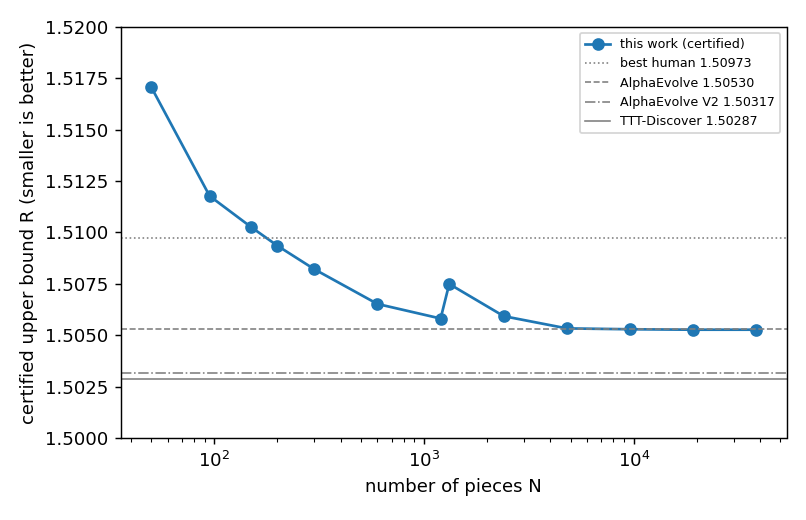
\includegraphics[width=.6\linewidth]{C_bound_vs_N.png}
\caption{Certified upper bound vs.\ number of pieces against the published bounds. Every point is a row of the table above except the isolated point at $N=1319$ ($R=1.507497$): that is a first-round \emph{from-scratch} run (GPU $p$-norm descent from 512 random restarts, then LP polish of the two best candidates, seed 11), not part of the re-melting ladder.}\label{fig:cbound}\end{figure}

\section{Limitations}
(i) The two sum-of-radii claims hold at a time stamp; the csqv table for $n\ge100$ changes hourly and either could be overtaken. (ii) The margins are small (relative $5.3\cdot10^{-5}$ and $2.4\cdot10^{-5}$). (iii) Only 20 values of $n\in[100,301]$ were attempted and the campaigns used a single workstation (12 cores, one 8\,GB GPU) for about a day of elapsed time (the 146 logged search runs in \texttt{results/runs} sum to 20.8\,h of per-run wall-clock, partly overlapping on the same machine; the Problem-C runs are not included in that sum). (iv) For $n\ne27,120,250$ we compared values, not coordinates. (v) The GPU modes and the melting schedules were only lightly tuned; CMA-ES/DE were piloted at one $n$. (vi) For problem C our best bound is above the later AI-discovered values, and we do not know whether those rely on a different structure. (vii) We did not re-verify other groups' certificates; reference values come from the cited sources on the stated dates. (viii) The GPU stage runs with \texttt{KMP\_DUPLICATE\_LIB\_OK=TRUE} on our Windows/conda installation to work around a duplicate OpenMP runtime; the verifier and CPU stages never import PyTorch. (ix) Packomania's homepage still stated on 2026-09-29 that submissions were closed (``over 5,000 new candidates in the queue''); nothing has been submitted.

\section{Reproducibility, data and code availability}\label{sec:repro}
\paragraph{Packomania data is not redistributed.} The repository, the Zenodo package and the Hugging Face dataset contain no Packomania table or coordinate file. \texttt{docs/packomania\_data.md} lists the URLs, retrieval times and SHA-256 checksums of the snapshots used here, and \texttt{python scripts/fetch\_packomania.py} downloads the files on demand into a git-ignored folder (checksums will usually differ from ours, because the tables change). Verification of our certificates and \texttt{.pck} files does not need them.
Everything needed to re-check the results is in the repository (code, certificates, \texttt{.pck} files, logs, tables, this paper): \texttt{pip install -r requirements.txt}; \texttt{make test}; \texttt{make verify} (re-verifies every certificate in fresh processes, both backends); \texttt{make reproduce} (rebuilds the headline table and figures from the certificates alone);
\texttt{python validator/validate\_pck.py submission/csqv120.pck submission/csqv250.pck}; \texttt{python -m search.record\_check} (time-stamped comparison with the live Packomania table). A clean \texttt{git clone} of the repository passes \texttt{make test} (51 tests), \texttt{make verify} (84 certificates, 168 checks) and \texttt{make reproduce}, and three further verification rounds with shuffled process order and different hash seeds gave identical results (\texttt{scripts/verify\_shuffled.py}; logs in \texttt{results/clean\_checkout\_20260929/}). Code: MIT licence; data and paper: CC-BY-4.0.
Archive: Zenodo DOI \href{https://doi.org/\zenododoi}{\texttt{\zenododoi}} (reserved; it resolves once the deposition is published); repository: \url{https://github.com/elianalfonsolopezpreciado/certified-packings}; dataset: \url{https://huggingface.co/datasets/elianalfonsolopezpreciado/certified-packings-data}.

\section*{AI-use disclosure}
The software implementation, automated testing, experiment execution and a first draft of the documentation were produced with Claude Code using the Claude Sonnet 5.5 model (Anthropic), under the direction of the author.
The author defined the research goals, chose the problems and methods to pursue, reviewed the results and the manuscript, and takes full responsibility for the content. The AI system is not an author.

\begin{thebibliography}{9}
\bibitem{packomania} E.~Specht, \emph{Packomania}. csqv: \url{https://www.packomania.com/csqv/csqv.html}, table \url{https://www.packomania.com/csqv/txt/sumradii.txt}; csq: \url{https://www.packomania.com/csq/}; submission hints: \url{http://www.packomania.com/hints.html}. Tables downloaded 2026-09-28 and 2026-09-29 (times stated in the text).
\bibitem{alphaevolve} A.~Novikov, N.~V\~u, M.~Eisenberger, E.~Dupont, et al., \emph{AlphaEvolve: A coding agent for scientific and algorithmic discovery}, arXiv:2506.13131 (2025).
\bibitem{tttdiscover} M.~Yuksekgonul, D.~Koceja, X.~Li, F.~Bianchi, J.~McCaleb, X.~Wang, J.~Kautz, Y.~Choi, J.~Zou, C.~Guestrin, Y.~Sun, \emph{Learning to Discover at Test Time}, arXiv:2601.16175 (v2, 2026); Tables~2 and~3, accessed 2026-09-29.
\end{thebibliography}
\end{document}
